\subsection{Kennzahlen}
    Nach jeder Klassifizierung wurden einige Kennzahlen des
    resultierenden Graphen ermittelt.
    Dies geschah im Fall einzelner Datenbanken und im Fall
    einer gemeinsamen.
    Zum besseren Verständnis der präsentierten Zahlen wird
    zunächst die konkrete Struktur der Graphen beschrieben.

    \paragraph{Struktur eines Graphen}
    Abbildung \ref{image:findingTeachersFiguresDbModel1}
    und \ref{image:findingTeachersFiguresDbModel2} zeigen,
    wie der Graph einer Klassifikation in diesem Fallbeispielt aufgebaut ist.
    Beide sind durch den \texttt{Content}-Knoten mit der Klasse \texttt{Teacher} verbunden.
    Referenzen sind in den Abbildungen nicht zu sehen,
    da sie lediglich Kanten von einem Knoten zu einer {\resource} darstellen
    und die Abbildungen unnötig vergrößern würden.
    Anhand des {\classificationModel}s und der beiden Abbildungen ist
    offensichtlich, welche Knoten Referenzen besitzen.
    Bei {\collectionFeature}s ist immer ein stellvertretendes Element zu sehen.

    \begin{figure}[htb]
        \centering
        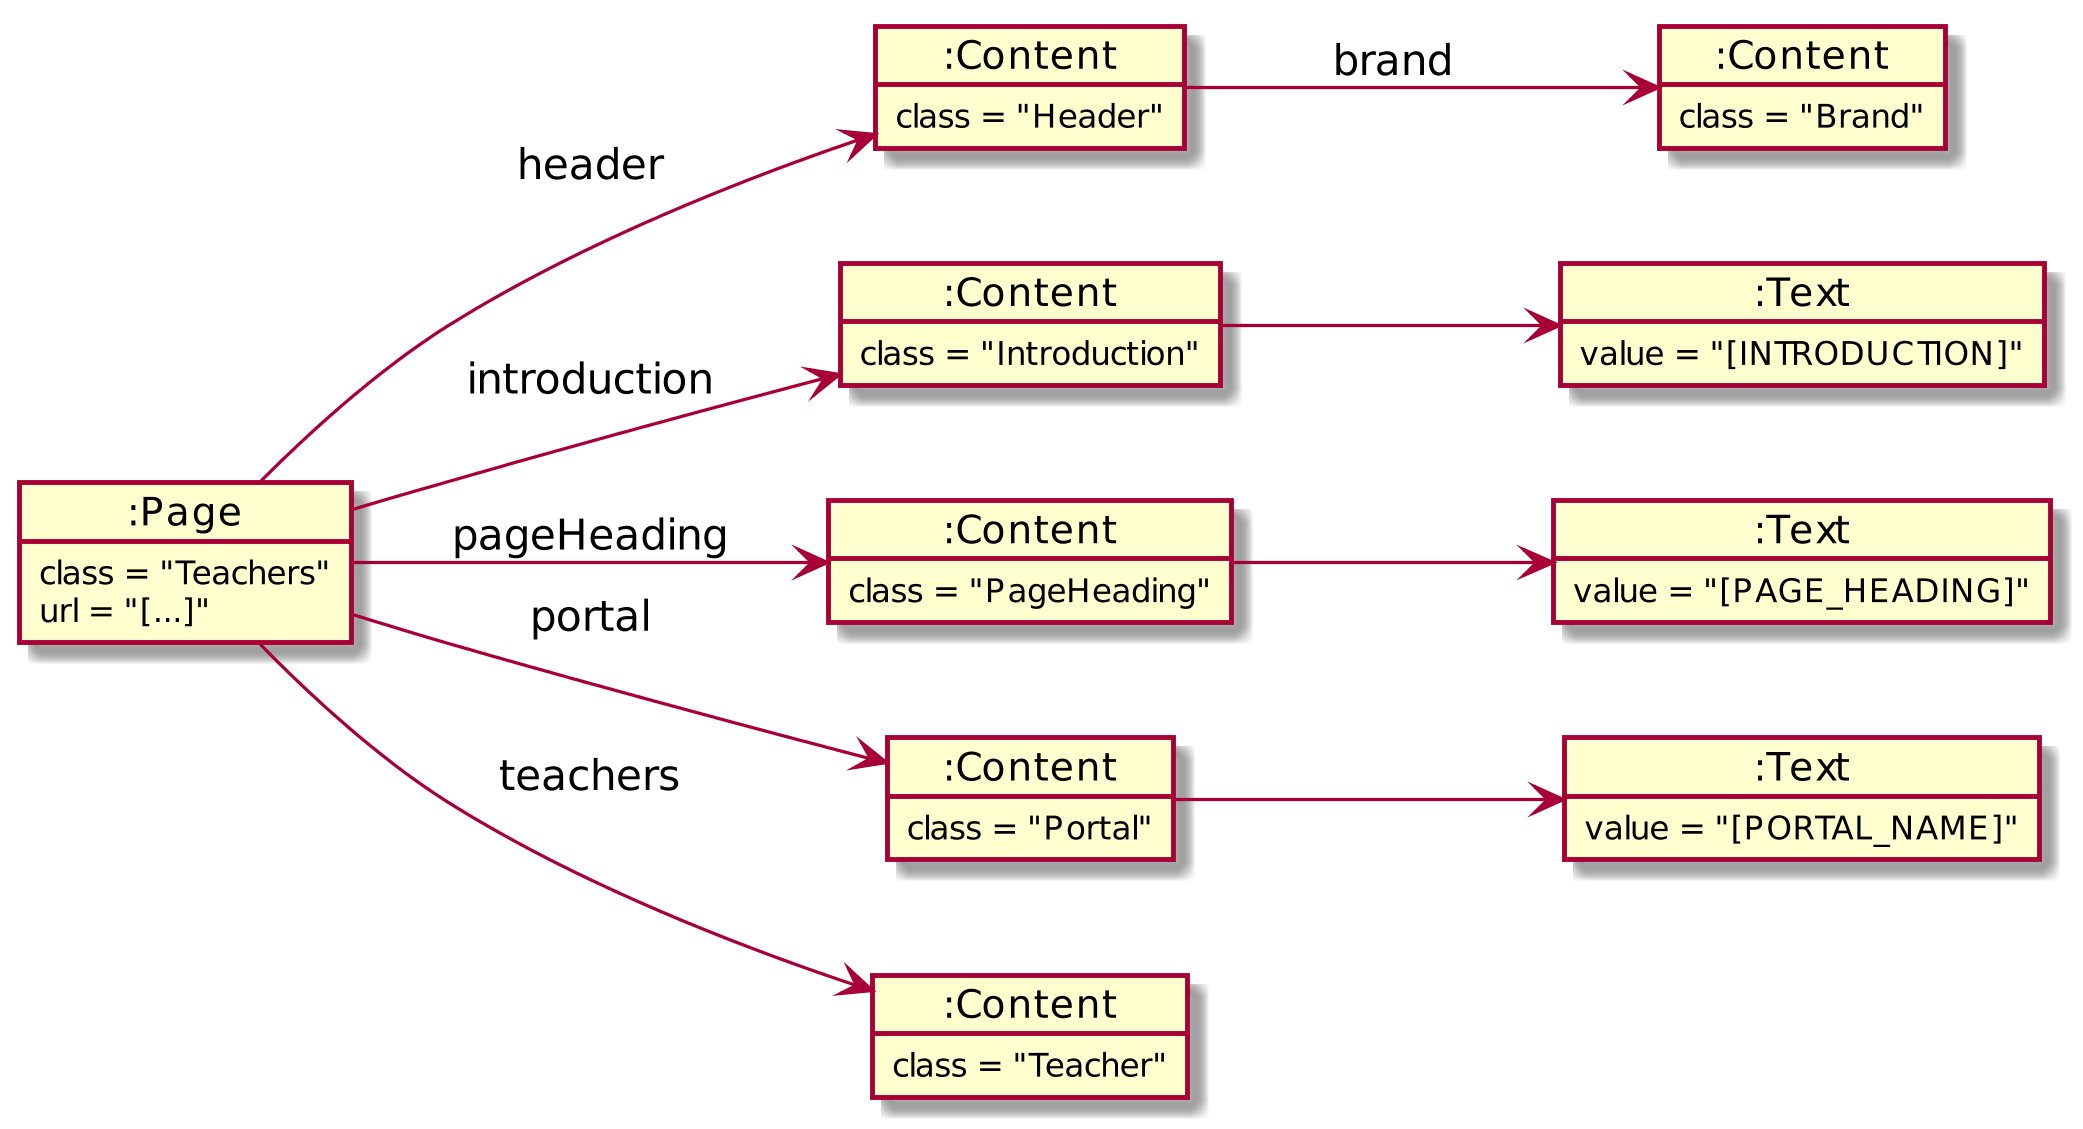
\includegraphics[scale=\imageScalingFactor]{../resources/findings/case-study-1/dbmodel/dbmodel1.png}
        \caption{Struktur des Graphen einer Seite über Lehrende und Betreuende (1)}
        \label{image:findingTeachersFiguresDbModel1}
    \end{figure}

    \begin{figure}[htb]
        \centering
        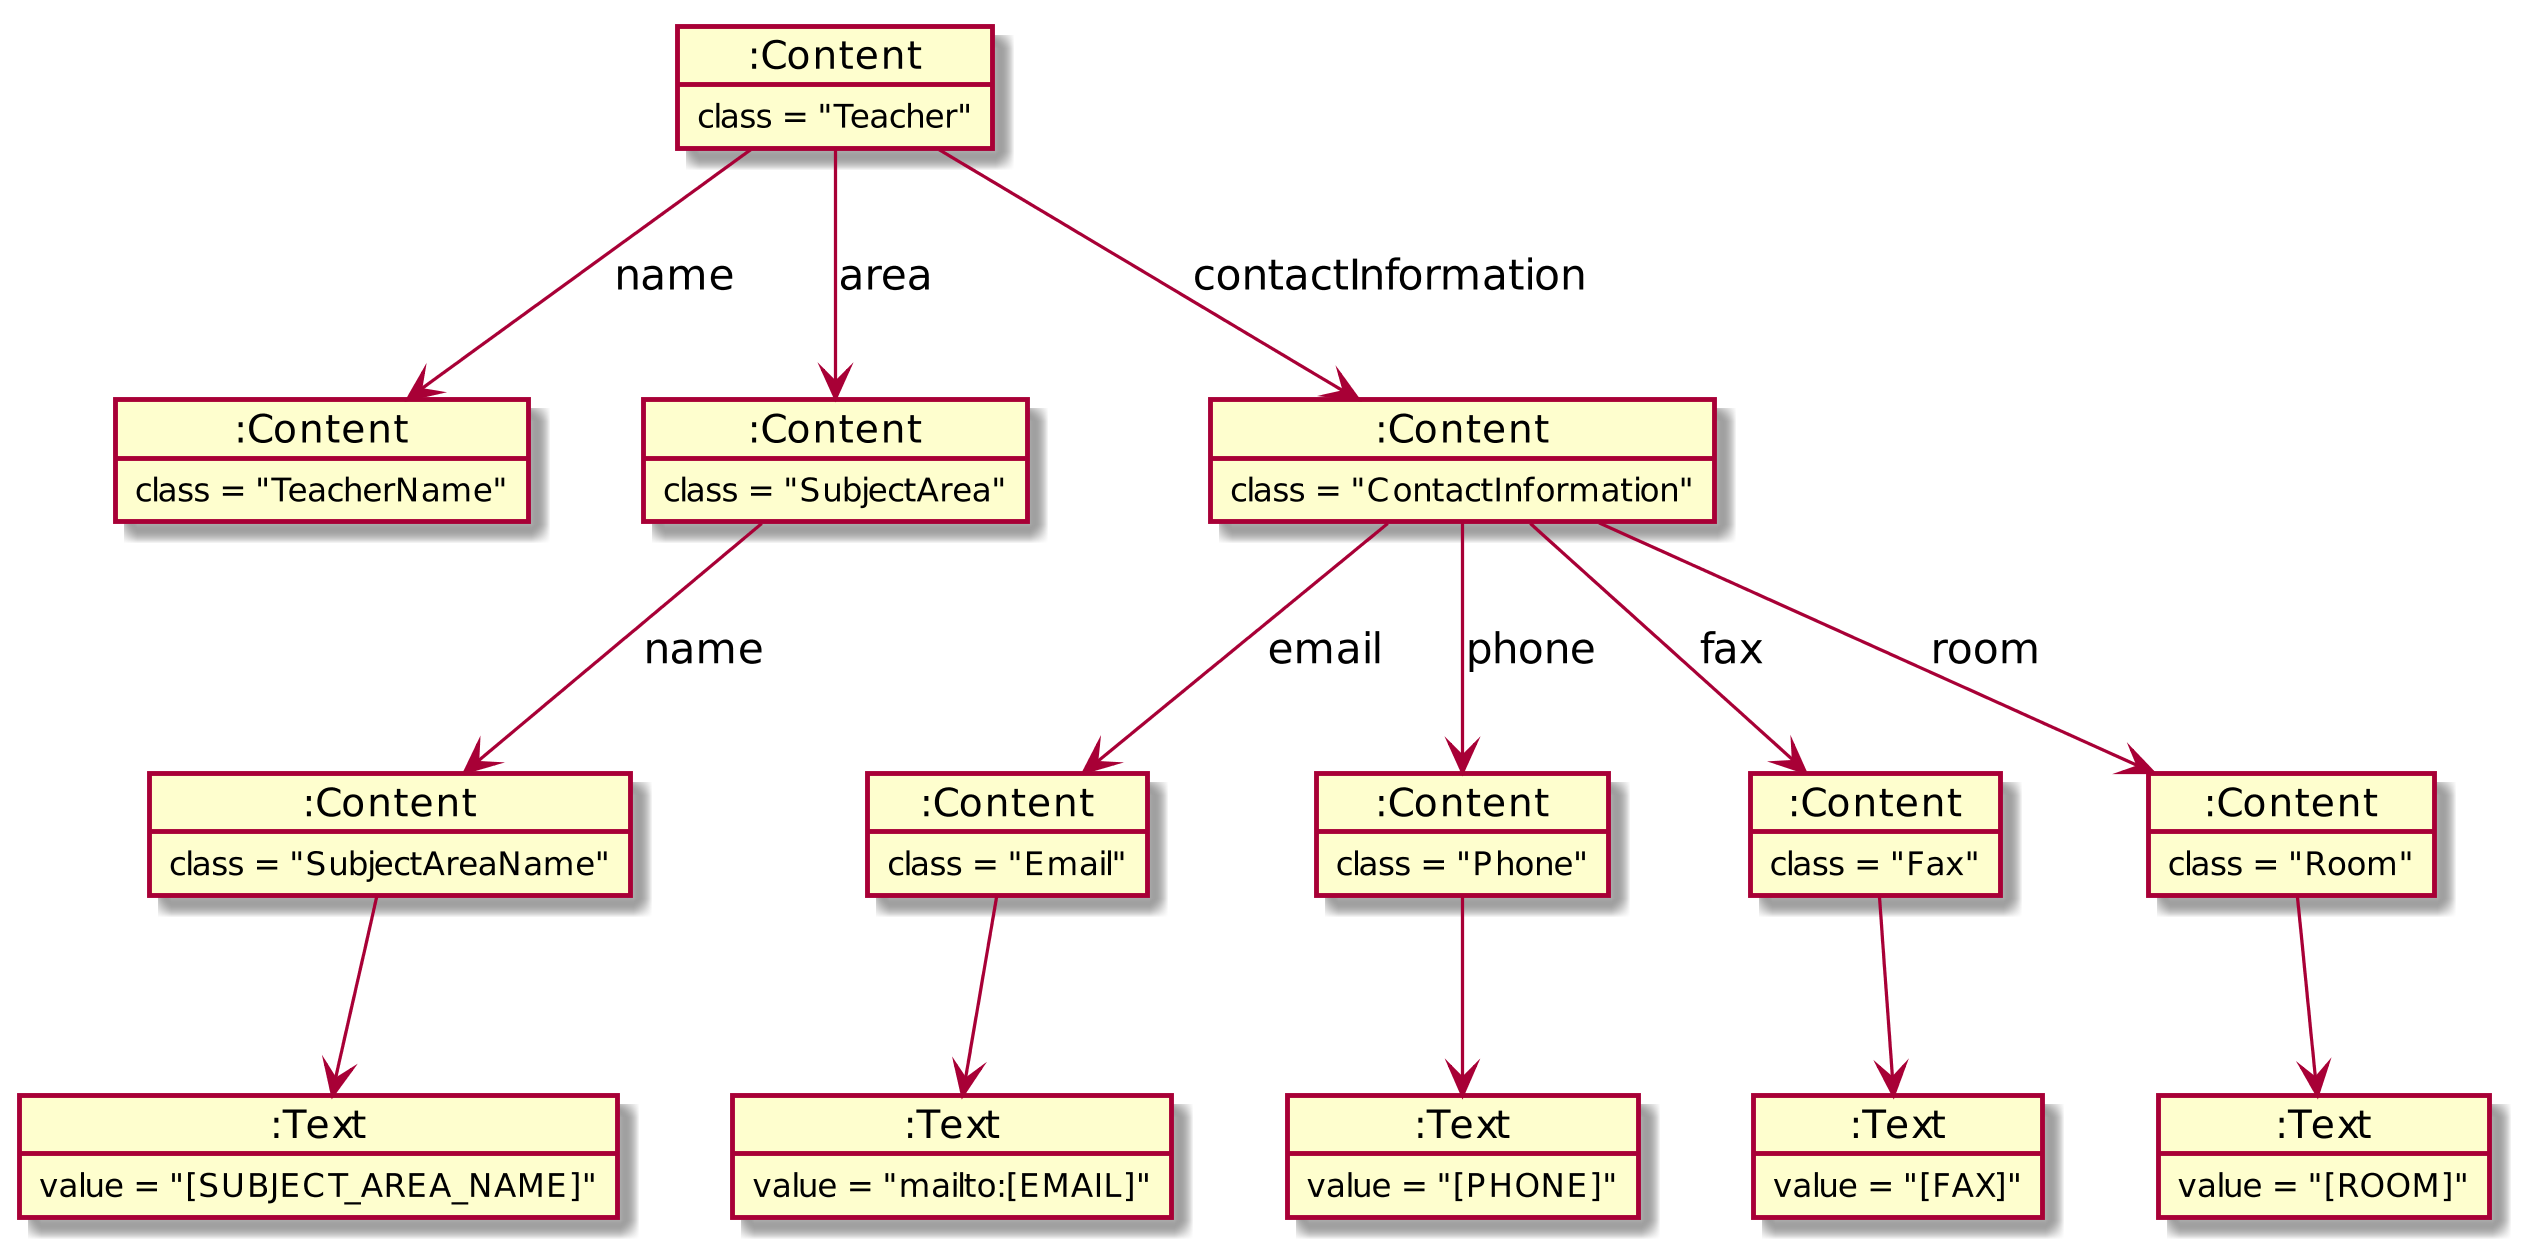
\includegraphics[scale=\imageScalingFactor]{../resources/findings/case-study-1/dbmodel/dbmodel2.png}
        \caption{Struktur des Graphen einer Seite über Lehrende und Betreuende (2)}
        \label{image:findingTeachersFiguresDbModel2}
    \end{figure}

    \paragraph{Präsentation der Kennzahlen}
    Die folgenden Tabellen präsentieren die gesammelten Kennzahlen.
    Sie sind folgendermaßen aufgebaut:
    Die erste Spalte benennt die Kennzahl.
    Dann folgen vier Spalten, die den Wert der Kennzahl für die einzelnen Portale enthalten.
    Diese Zahlen werden in der Spalte "`Summe"' aufaddiert,
    um sie mit der letzten Spalte zu vergleichen.
    Diese gibt den Wert der Kennzahl für den Fall der gemeinsam genutzten Datenbank an.
    Eine ausführliche Interpretation dieser Zahlen geschieht in Kapitel \ref{section:findingsInterpretation}.
    Trotzdem wird hier schon die Bedeutung einiger Kennzahlen kurz hervorgehoben.

    Tabelle \ref{table:findingsTeachersFiguresNodesByLabel}
    gruppiert die Knoten der Datenbank nach ihren Labels und zeigt,
    wie oft jedes Label oder jede Kombination von Labels Verwendung fand.   
    Für die einzelnen Klassifikationen gibt \texttt{Content} außerdem an,
    wie viele {\contentFeature}s sie enthalten.

    \begin{table}[htb]
        \centering
        \begin{tabular}{|l|c|c|c|c|c|c|}
            \hline
            \multicolumn{1}{|c|}{\textbf{Label}} & \textbf{\gls{babw}} & \textbf{\gls{bapvs}} & \textbf{\gls{bscpsy}} & \textbf{\gls{mabm}} & \textbf{Summe} & \textbf{Alle} \\ \hline
            \texttt{Content}                                     & 270           & 275            & 176             & 128           & 849            & 824           \\ \hline
            \texttt{Page} + \texttt{Resource}                             & 1             & 1              & 1               & 1             & 4              & 4             \\ \hline
            \texttt{Resource}                                    & 133           & 159            & 89              & 71            & 452            & 430           \\ \hline
            \texttt{Site}                                        & 1             & 1              & 1               & 1             & 4              & 4             \\ \hline
            \texttt{Text}                                        & 105           & 69             & 75              & 56            & 305            & 284           \\ \hline
            \hline
            \textbf{Summe}                              & 510           & 505            & 342             & 257           & 1614           & 1546          \\ \hline
        \end{tabular}
        \caption{Knoten gruppiert nach Labels für Seiten über Lehrende und Betreuende}
        \label{table:findingsTeachersFiguresNodesByLabel}
    \end{table}

    Die Knoten mit dem Label \texttt{Content} lassen sich nach der ihnen zugewiesenen Klasse
    weiter aufschlüssen, was in Tabelle \ref{table:findingsTeachersFiguresContentNodesByClass} geschieht.
    Eine Kennzahl in dieser Tabelle ist gleichzusetzen mit der Häufigkeit der Verwendung
    der genannten Klasse in der Klassifikation.

    \begin{table}[htb]
        \centering
        \begin{tabular}{|l|c|c|c|c|c|c|}
        \hline
            \textbf{Klasse}  & \multicolumn{1}{l|}{\textbf{\gls{babw}}} & \multicolumn{1}{l|}{\textbf{\gls{bapvs}}} & \multicolumn{1}{l|}{\textbf{\gls{bscpsy}}} & \multicolumn{1}{l|}{\textbf{\gls{mabm}}} & \multicolumn{1}{l|}{\textbf{Summe}} & \multicolumn{1}{l|}{\textbf{Alle}} \\ \hline
            \texttt{Brand}              & 1                                  & 1                                   & 1                                    & 1                                  & 4                                   & 4                                  \\ \hline
            \texttt{ContactInformation} & 55                                 & 67                                  & 33                                   & 24                                 & 179                                 & 178                                \\ \hline
            \texttt{Fax}                & 1                                  & 0                                   & 0                                    & 1                                  & 2                                   & 1                                  \\ \hline
            \texttt{Header}             & 1                                  & 1                                   & 1                                    & 1                                  & 4                                   & 4                                  \\ \hline
            \texttt{Introduction}       & 1                                  & 0                                   & 1                                    & 1                                  & 3                                   & 2                                  \\ \hline
            \texttt{PageHeading}        & 1                                  & 1                                   & 1                                    & 1                                  & 4                                   & 4                                  \\ \hline
            \texttt{Phone}              & 35                                 & 38                                  & 29                                   & 21                                 & 123                                 & 119                                \\ \hline
            \texttt{Portal}             & 1                                  & 1                                   & 1                                    & 1                                  & 4                                   & 4                                  \\ \hline
            \texttt{Room}               & 2                                  & 0                                   & 0                                    & 0                                  & 2                                   & 2                                  \\ \hline
            \texttt{SubjectArea}        & 53                                 & 67                                  & 33                                   & 22                                 & 175                                 & 172                                \\ \hline
            \texttt{SubjectAreaName}    & 9                                  & 18                                  & 11                                   & 7                                  & 45                                  & 39                                 \\ \hline
            \texttt{Teacher}            & 55                                 & 70                                  & 33                                   & 24                                 & 182                                 & 182                                \\ \hline
            \texttt{TeacherName}        & 55                                 & 11                                  & 32                                   & 24                                 & 122                                 & 113                                \\ \hline
            \hline
            \textbf{Summe}     & 270                                & 275                                 & 176                                  & 128                                & 849                                 & 824                                \\ \hline
        \end{tabular}
        \caption{\texttt{Content}-Knoten gruppiert nach ihrer Klasse für Seiten über Lehrende und Betreuende}
        \label{table:findingsTeachersFiguresContentNodesByClass}
    \end{table}

    Auch über die Kanten der Graphen lassen sich einige Zahlen ermitteln.
    Tabelle \ref{table:findingTeachersFiguresEdgesByLabel} beginnt dazu
    mit der Aufschlüsselung der Kanten nach ihrem Label.
    Die Kennzahl \texttt{References} spiegelt die Anzahl der Referenzen innerhalb einer Klassifikation wieder.

    \begin{table}[htb]
        \centering
        \begin{tabular}{|l|c|c|c|c|c|c|}
            \hline
            \multicolumn{1}{|c|}{\textbf{Kanten-Label}} & \textbf{\gls{babw}} & \textbf{\gls{bapvs}} & \textbf{\gls{bscpsy}} & \textbf{\gls{mabm}} & \textbf{Summe} & \textbf{Alle} \\ \hline
            \texttt{Reads}                                       & 105           & 69             & 75              & 56            & 305            & 284           \\ \hline
            \texttt{References}                                  & 180           & 209            & 110             & 86            & 585            & 582           \\ \hline
            \texttt{Owns}                                        & 320           & 335            & 200             & 144           & 999            & 996           \\ \hline
            \hline
            \textbf{Summe}                              & 605           & 613            & 385             & 286           & 1889           & 1862          \\ \hline
        \end{tabular}
        \caption{Kanten gruppiert nach Labels für Seiten über Lehrende und Betreuende}
        \label{table:findingTeachersFiguresEdgesByLabel}
    \end{table}

    Neben dem Label ist in Bezug auf Kanten auch die Frage interessant,
    welche Knoten sie verbinden.
    Tabelle \ref{table:findingsTeachersFiguresEdgesByStartEndNodeLabel}
    zeigt, welche Arten von Knoten wie oft mit einander verbunden wurden.
    Die Beziehung eines \texttt{Content}-Knotens zu einem \texttt{Text}-Knoten
    zeigt die Übersicht nicht,
    da sie äquivalent zum zuvor gezeigten \texttt{Reads}-Label ist.
    Tabelle \ref{table:findingsTeachersFiguresEdgesByStartEndNodeLabel} gibt dadurch unter anderem Aufschluss über die Zahl der Referenzen
    einer Seite bzw. von {\contentFeature}s.

    \begin{table}[htb]
        \centering
        \begin{tabular}{|l|c|c|c|c|c|c|}
            \hline
            \multicolumn{1}{|c|}{\textbf{Labels verbundener Knoten}} & \textbf{\gls{babw}} & \textbf{\gls{bapvs}} & \textbf{\gls{bscpsy}} & \textbf{\gls{mabm}} & \textbf{Summe} & \textbf{Alle} \\ \hline
            \texttt{(:Content)} $\rightarrow$ \texttt{(:Content)}                           & 260           & 260            & 162             & 115           & 797            & 794           \\ \hline
            \texttt{(:Content)} $\rightarrow$ \texttt{(:Resource)}                         & 172           & 201            & 102             & 78            & 553            & 550           \\ \hline
            \texttt{(:Page)} $\rightarrow$ \texttt{(:Content)}                              & 59            & 74             & 37              & 28            & 198            & 198           \\ \hline
            \texttt{(:Page)} $\rightarrow$ \texttt{(:Resource)}                             & 8             & 8              & 8               & 8             & 32             & 32            \\ \hline
            \texttt{(:Site)} $\rightarrow$ \texttt{(:Page)}                                 & 1             & 1              & 1               & 1             & 4              & 4             \\ \hline
            \hline
            \textbf{Summe}                                          & 500           & 544            & 310             & 230           & 1584           & 1578          \\ \hline
        \end{tabular}
        \caption{Kanten gruppiert nach Labels der Start- und Zielknoten für Seiten über Lehrende und Betreuende}
        \label{table:findingsTeachersFiguresEdgesByStartEndNodeLabel}
    \end{table}

    Eine letzte zu beantwortende Frage ist,
    wie viele Knoten in der Datenbank mehr als eine eingehende Kante haben.
    Bei mehr als einer Kante findet ein Knoten an verschiedenen Stellen 
    einer oder mehrerer Klassifikationen Verwendung.
    Entsprechende Zahlen bietet Tabelle \ref{table:findingsTeachersFiguresSharedNodes},
    deren erste Spalte die Klasse eines \texttt{Content}-Knotens oder
    die Art einer {\resource} beschreibt.

    \begin{table}[htb]
        \centering
        \begin{tabular}{|l|c|c|c|c|c|c|}
            \hline
            \multicolumn{1}{|c|}{\textbf{Knoten}} & \textbf{\gls{babw}} & \textbf{\gls{bapvs}} & \textbf{\gls{bscpsy}} & \textbf{\gls{mabm}} & \textbf{Summe} & \textbf{Alle} \\ \hline
            Bild eines Mitarbeiters                                  & 0             & 1              & 1               & 0             & 2              & 2             \\ \hline
            \texttt{ContactInformation}                    & 0             & 3              & 0               & 0             & 3              & 3             \\ \hline
            E-Mail-Adresse                        & 0             & 1              & 1               & 0             & 2              & 14            \\ \hline
            \texttt{Fax}                                   & 0             & 0              & 0               & 0             & 0              & 1             \\ \hline
            Hauptseite "`Studium"'                & 1             & 0              & 0               & 0             & 1              & 1             \\ \hline
            Homepage der FU                       & 0             & 0              & 0               & 0             & 0              & 1             \\ \hline
            \texttt{Introduction}                          & 0             & 0              & 0               & 0             & 0              & 1             \\ \hline
            Lehrgebietsseiten                     & 7             & 16             & 8               & 5             & 36             & 30            \\ \hline
            \texttt{Phone}                                 & 4             & 1              & 0               & 0             & 5              & 9             \\ \hline
            \texttt{SubjectArea}                           & 0             & 2              & 0               & 0             & 2              & 5             \\ \hline
            \texttt{SubjectAreaName}                       & 8             & 16             & 7               & 5             & 36             & 31            \\ \hline
            \texttt{Teacher}                               & 0             & 1              & 0               & 0             & 1              & 1             \\ \hline
            \texttt{TeacherName}                           & 0             & 3              & 1               & 0             & 4              & 13            \\ \hline
            \hline
            \textbf{Summe}                        & 20            & 44             & 18              & 10            & 92             & 112           \\ \hline
        \end{tabular}
        \caption{Knoten mit mehreren eingehenden Kanten für Seiten über Lehrende und Betreuende}
        \label{table:findingsTeachersFiguresSharedNodes}
    \end{table}
